\documentclass[11pt]{article}
\usepackage{amsmath,amssymb,amsthm,mathtools}
\usepackage[margin=1in]{geometry}
\usepackage{algorithm}
\usepackage{algpseudocode}
\usepackage{xcolor}
\usepackage{graphicx}
\usepackage{booktabs,tabularx}
\usepackage{enumitem}
\usepackage[font=small,labelfont=bf]{caption}
\usepackage{microtype}
\usepackage{array}
\usepackage{upquote}
\usepackage[section]{placeins}
\usepackage[colorlinks=true,linkcolor=blue!50!black,citecolor=blue!50!black,urlcolor=blue!50!black]{hyperref}

\newtheorem{theorem}{Theorem}[section]
\newtheorem{lemma}[theorem]{Lemma}
\newtheorem{proposition}[theorem]{Proposition}
\theoremstyle{plain}
\newtheorem{assumption}{Assumption}

\DeclareMathOperator{\Null}{Null}
\DeclareMathOperator{\Range}{Range}

\title{The Recursive Complete Minimum-Norm HSS Solver\\[2pt]
\large algorithm, proof of optimality, and numerical experiments}
\author{Arjun Sethi-Olowin}
\date{October 2026}

% generated by make_figures.py from ../../hss_examples/minnorm_paper/results
% 25.2.0.3177638 (R2025b) Update 5 | MACA64 | threads 10 | 02-Oct-2026 16:24:17
% 25.2.0.3177638 (R2025b) Update 5 | MACA64 | threads 10 | 02-Oct-2026 16:25:18
% 25.2.0.3177638 (R2025b) Update 5 | MACA64 | threads 10 | 02-Oct-2026 16:00:39
\newcommand{\EoneMaxRes}{7.7\times10^{-14}}
\newcommand{\EoneMaxErr}{1.9\times10^{-13}}
\newcommand{\EoneMaxNull}{1.9\times10^{-13}}
\newcommand{\EoneMaxErrOverKappaU}{14}
\newcommand{\EoneSmallKappaClause}{; the largest ratios occur for $\kappa(H)<10$, where the solver error is at most $4.2\times10^{-15}$}
\newcommand{\EoneCompMin}{1.0\times10^{-12}}
\newcommand{\EoneCompMax}{6.7\times10^{-11}}
\newcommand{\EoneNoSlack}{F2 $m/n=0.9$, F5 and F6}
\newcommand{\EtwoUlvOverKappaU}{3}
\newcommand{\EtwoMaxKappaGraded}{1.8\times10^{13}}
\newcommand{\EtwoMaxKappaBlur}{1.1\times10^{8}}
\newcommand{\EtwoUlvBwdMax}{3.5\times10^{-16}}
\newcommand{\EtwoQrBwdMax}{2.2\times10^{-16}}
\newcommand{\EtwoNeBwdMax}{1.0\times10^{-8}}
\newcommand{\EtwoCholFailGraded}{1.7\times10^{9}}
\newcommand{\EtwoCgFailGraded}{9.8\times10^{3}}
\newcommand{\EtwoCgItsMinGraded}{99}
\newcommand{\EtwoCholFailBlur}{1.1\times10^{8}}
\newcommand{\EtwoCgFailBlur}{6.1\times10^{2}}
\newcommand{\EtwoCgItsMinBlur}{47}
\newcommand{\EfourSlopeMin}{0.97}
\newcommand{\EfourSlopeMax}{1.05}
\newcommand{\EfourSlopeRepeatMin}{0.97}
\newcommand{\EfourSlopeRepeatMax}{1.04}
\newcommand{\EfourRatioRepeat}{25--46}
\newcommand{\EfourRepeatMatvec}{2--3}
\newcommand{\EfourMaxN}{2^{17}}
\newcommand{\EfourDenseN}{8192}
\newcommand{\EfourDenseRatio}{38}
\newcommand{\EfourDenseSlope}{2.6}
\newcommand{\EfourCgN}{32768}
\newcommand{\EfourCgRatio}{6}
\newcommand{\EfourCgRatioRepeat}{150}
\newcommand{\EfourCgIts}{79--171}
\newcommand{\EthreeMaxRes}{2.8\times10^{-15}}
\newcommand{\EthreeErrMin}{1.7\times10^{-15}}
\newcommand{\EthreeErrMax}{5.6\times10^{-15}}
\newcommand{\EthreeFoneFirst}{7.8\times10^{-14}}
\newcommand{\EthreeFoneLast}{5.6\times10^{-12}}
\newcommand{\EthreeFoneN}{2^{17}}
\newcommand{\KFone}{$10^{3}$--$7{\times}10^{3}$}
\newcommand{\KFtwo}{$13$--$79$}
\newcommand{\KFthree}{$\approx1.9$}
\newcommand{\KFfive}{$\approx2.0$}
\newcommand{\KFsix}{$\approx7.4$}
\newcommand{\KFtwoG}{$9.3$--$2{\times}10^{13}$}
\newcommand{\KFfour}{$3.0$--$10^{8}$}
\newcommand{\TimingPlatform}{MATLAB R2025b (Apple silicon Mac, 10 threads)}
\newcommand{\PlatformSentence}{All results were computed with \TimingPlatform.}


\begin{document}
\maketitle

\section{Introduction}
These notes describe a direct, ULV-type algorithm that computes the minimum-norm solution
$x^\star=H^+b$ of $Hx=b$, where $H$ is a wide (or square) hierarchically semiseparable (HSS) matrix of
full row rank. The algorithm works one tree level at a time: unitary transformations decouple part of the
unknowns of every leaf, those unknowns are solved for directly, and what remains is a smaller HSS system
with one level fewer. We prove that the result is exactly $H^+b$ and that the cost is linear in $n$, and
test the algorithm numerically.
\begin{itemize}[leftmargin=1.4em,itemsep=1pt]
\item Section~\ref{sec:setup}: notation and the one standing assumption on the representation.
\item Section~\ref{sec:algorithm}: one level of the algorithm (size reduction, decoupling, forced solve,
reduced matrix, reconstruction), and why the slack condition of the fixed-width formulation is not needed.
\item Section~\ref{sec:proof}: proof that the algorithm returns $H^+b$: four lemmas, one level, all levels.
\item Section~\ref{sec:complexity}: complexity, with measured times.
\item Section~\ref{sec:summary}: the algorithm in pseudocode.
\item Section~\ref{sec:numerics}: numerical experiments: test matrices, correctness against dense
solutions, accuracy as the condition number grows, accuracy at large $n$.
\item Section~\ref{sec:open}: open problems.
\end{itemize}

% ======================================================================
\section{Setup and Notation}
\label{sec:setup}

We consider a matrix $H\in\mathbb{C}^{m\times n}$, $m\le n$, of full row rank, given in HSS form, and want
\[
x^\star=\operatorname*{arg\,min}_{Hx=b}\|x\|_2 = H^*(HH^*)^{-1}b = H^+ b .
\]
For $m=n$ this is the solution $H^{-1}b$; the algorithm covers both cases.

\paragraph{Tree and generators.}
$\mathcal T$ is a perfect binary tree of depth $L$. Node $\tau$ owns a row index set
$I_\tau$ and a column index set $J_\tau$, and the children of a node partition its index
sets. For a \emph{leaf} $\tau$,
\[
D_\tau = H(I_\tau,J_\tau)\in\mathbb{C}^{n_\tau\times p_\tau},\qquad
U_\tau\in\mathbb{C}^{n_\tau\times k_\tau},\qquad
V_\tau\in\mathbb{C}^{p_\tau\times \ell_\tau}:
\]
a leaf has $n_\tau$ rows and $p_\tau$ columns, $k_\tau$ is the rank of its row basis and $\ell_\tau$
the rank of its column basis. (So $n_\tau$ counts the \emph{rows} of a leaf, while $n$ counts the
\emph{columns} of $H$.) A non-leaf, non-root node $\pi$ with children $\alpha,\beta$ stores translation
matrices $R_\pi\in\mathbb{C}^{(k_\alpha+k_\beta)\times k_\pi}$ and
$W_\pi\in\mathbb{C}^{(\ell_\alpha+\ell_\beta)\times\ell_\pi}$, and the nested bases are
\[
\mathbf U_\tau = U_\tau,\ \mathbf V_\tau=V_\tau\ (\tau\text{ a leaf}),\qquad
\mathbf U_\pi=\begin{bmatrix}\mathbf U_\alpha&\\&\mathbf U_\beta\end{bmatrix}R_\pi,\qquad
\mathbf V_\pi=\begin{bmatrix}\mathbf V_\alpha&\\&\mathbf V_\beta\end{bmatrix}W_\pi .
\]
For siblings $\alpha,\beta$ (children of the same node),
\begin{equation}\label{eq:offdiag}
H(I_\alpha,J_\beta)=\mathbf U_\alpha B_{\alpha\beta}\mathbf V_\beta^*,\qquad B_{\alpha\beta}\in\mathbb{C}^{k_\alpha\times\ell_\beta}.
\end{equation}
Unrolling the nested bases, the part of leaf $\tau$'s block row outside its diagonal block is
$H(I_\tau,J\setminus J_\tau)=U_\tau G_\tau$, and the part of its block column outside the diagonal
block is $H(I\setminus I_\tau,J_\tau)=F_\tau V_\tau^*$, for some matrices $G_\tau,F_\tau$. Consequently,
a unitary transformation of the rows of leaf $\tau$ acts on its whole block row through $U_\tau$
and $D_\tau$ alone, and a unitary transformation of its columns acts on its whole block column
through $V_\tau$ and $D_\tau$ alone. This is what makes the leaf-local operations below global.

\paragraph{Proper representation.} We assume that no basis is wider than the block it spans:
$k_\tau\le n_\tau$ for every leaf, and $k_\pi\le k_\alpha+k_\beta$ for every non-leaf $\pi$ with children
$\alpha,\beta$. This is a property of the representation, not of $H$: any representation can be
brought to this form without changing $H$ (replace a wide basis by an orthonormal basis of its
range and absorb the remaining factor into the parent's translation and into $B$), and
nested-basis constructions produce it directly. The algorithm uses it only so that the number of
decoupled rows $t_\tau=n_\tau-k_\tau$ in Section~\ref{subsec:decoupling} is nonnegative.

\paragraph{Right compressions and QL factorizations.} For $M\in\mathbb{C}^{a\times p}$, $a\le p$, a
\emph{right compression} is a unitary $Q\in\mathbb{C}^{p\times p}$ with $MQ=[L,\;0]$,
$L\in\mathbb{C}^{a\times a}$ lower triangular; it comes from a QR factorization
$M^*=Q\begin{bmatrix}R\\0\end{bmatrix}$, $L=R^*$. A \emph{QL factorization} of a tall
$U\in\mathbb{C}^{n\times k}$ ($k\le n$) is $U=P\begin{bmatrix}0\\ \hat U\end{bmatrix}$ with $P$ unitary
and $\hat U\in\mathbb{C}^{k\times k}$ lower triangular.

% ======================================================================
\section{One Level of the Algorithm}
\label{sec:algorithm}

The algorithm is a minimum-norm variant of the ULV elimination of~\cite{cgp}. One level processes
every leaf $\tau$ independently and then forms a reduced HSS system with one level fewer, which is
solved recursively. We list the operations for a leaf $\tau$ with parent $\pi$ and sibling $\sigma$.

\subsection{Size reduction}\label{subsec:sizereduction}
If $\ell_\tau+n_\tau<p_\tau$, compute a unitary $\Omega_\tau$ (from a QR factorization of the
$p_\tau\times(\ell_\tau+n_\tau)$ matrix $[V_\tau,\ D_\tau^*]$) with
\begin{equation}\label{eq:sizered}
\begin{bmatrix}V_\tau^*\\ D_\tau\end{bmatrix}\Omega_\tau=
\begin{bmatrix}\tilde V_\tau^* & 0\\ \tilde D_\tau & 0\end{bmatrix},\qquad
\tilde V_\tau^*\in\mathbb{C}^{\ell_\tau\times p_\tau'},\quad \tilde D_\tau\in\mathbb{C}^{n_\tau\times p_\tau'},
\end{equation}
where $p'_\tau=\ell_\tau+n_\tau$. Otherwise there is nothing to remove: $\Omega_\tau=I$ and
$p'_\tau=p_\tau$. In both cases $p'_\tau=\min(p_\tau,\ell_\tau+n_\tau)$. Every row of $H(:,J_\tau)$ is a
combination of the rows of $[V_\tau^*;D_\tau]$ (Section~\ref{sec:setup}), so the last $p_\tau-p'_\tau$
columns of $H(:,J_\tau)\Omega_\tau$ vanish in every block row. Dropping them gives $\tilde H$: the same
tree and generators, except $D_\tau\to\tilde D_\tau$ and $V_\tau\to\tilde V_\tau$.

\begin{assumption}[slack]\label{as:slack}
Every leaf satisfies $\ell_\tau+n_\tau\le p_\tau$.
\end{assumption}
\noindent Under Assumption~\ref{as:slack} the size reduction removes $p_\tau-\ell_\tau-n_\tau\ge0$ columns from
every leaf and leaves exactly $p'_\tau=\ell_\tau+n_\tau$, so all block sizes are known in advance; a
formulation with this fixed width needs the assumption. The algorithm itself does not, for two
reasons.
\begin{enumerate}[leftmargin=1.5em,itemsep=1pt]
\item The size reduction only discards columns along which $H$ vanishes identically. When
$\ell_\tau+n_\tau\ge p_\tau$ there may be none, and $\Omega_\tau=I$. Lemma~\ref{lem:orthogonal} below, which
justifies the step, holds with an empty set of discarded columns.
\item After the size reduction, the sizes enter at exactly one point: the forced block $L_\tau$ of
Section~\ref{subsec:decoupling} must be square, which requires $t_\tau\le p'_\tau$. This follows from
full row rank alone (Lemma~\ref{lem:rank}): the $t_\tau$ decoupled rows of leaf $\tau$ are nonzero only
in $\tau$'s $p'_\tau$ columns, and the rows of a full-row-rank matrix are linearly independent.
\end{enumerate}
Without the assumption, a reduced leaf has $f_\tau=p'_\tau-t_\tau$ free columns, which can be fewer
than its $k_\tau$ coupled rows; reduced leaves can then be square or tall. Only the reduced matrix as a
whole has to have full row rank, and Lemma~\ref{lem:rank} shows that it does.

\subsection{Decoupling}\label{subsec:decoupling}
\paragraph{Step 1 (row compression).} QL-factor $U_\tau=P_\tau\begin{bmatrix}0\\ \hat U_\tau\end{bmatrix}$
and multiply $\tau$'s rows (of $\tilde D_\tau$ and of $b$) by $P_\tau^*$. With $t_\tau:=n_\tau-k_\tau$, the
top $t_\tau$ rows of $P_\tau^*U_\tau$ are zero, so the top $t_\tau$ rows of $\tau$'s block row vanish
outside $J_\tau$.

\paragraph{Step 2 (column decoupling).} Right-compress the top rows,
$(P_\tau^*\tilde D_\tau)(1{:}t_\tau,:)\,Q_\tau=[L_\tau,\;0]$, with $L_\tau\in\mathbb{C}^{t_\tau\times t_\tau}$
lower triangular and $Q_\tau\in\mathbb{C}^{p_\tau'\times p_\tau'}$ unitary (this needs $t_\tau\le p'_\tau$, which
holds by Lemma~\ref{lem:rank}), and apply $Q_\tau$ to all of $\tau$'s columns:
\begin{equation}\label{eq:decoupled}
\hat D_\tau:=P_\tau^*\tilde D_\tau Q_\tau=\begin{bmatrix}L_\tau & 0\\ C_\tau & E_\tau\end{bmatrix},\qquad
\hat V_\tau^*:=\tilde V_\tau^*Q_\tau=\begin{bmatrix}\hat V_{\tau,1}^* & \hat V_{\tau,2}^*\end{bmatrix},
\end{equation}
with $C_\tau\in\mathbb{C}^{k_\tau\times t_\tau}$ and $E_\tau\in\mathbb{C}^{k_\tau\times f_\tau}$,
$f_\tau=p_\tau'-t_\tau$. Write $\hat H=P^*\tilde HQ$ and $\hat b=P^*b$, with
$P=\operatorname{diag}(P_\tau)$ and $Q=\operatorname{diag}(Q_\tau)$.

\paragraph{Zero pattern.} Split the rows of each leaf into the top $t_\tau$ (\emph{decoupled} rows,
set $\mathcal R_1$) and the bottom $k_\tau$ ($\mathcal R_2$), and its columns into the first $t_\tau$
(\emph{forced} columns, $\mathcal C_1$) and the remaining $f_\tau$ (\emph{free} columns, $\mathcal C_2$).
Then
\begin{equation}\label{eq:blocktri}
\hat H=\begin{bmatrix}\hat H(\mathcal R_1,\mathcal C_1)&\hat H(\mathcal R_1,\mathcal C_2)\\ \hat H(\mathcal R_2,\mathcal C_1)&\hat H(\mathcal R_2,\mathcal C_2)\end{bmatrix}
=\begin{bmatrix}\mathbf L & 0\\ M & \bar H\end{bmatrix},\qquad \mathbf L=\operatorname{diag}(L_\tau).
\end{equation}
$\hat H(\mathcal R_1,\mathcal C_1)$ is block diagonal because a decoupled row of $\tau$ is zero in every other
leaf's columns (Step~1), and $\hat H(\mathcal R_1,\mathcal C_2)=0$ because, in addition, it is zero in $\tau$'s
own free columns (Step~2).

\subsection{Forced solve and the reduced right-hand side}\label{subsec:forcedsolve}
Write $\hat x_\tau=[X^{(1)}_\tau;X^{(2)}_\tau]$ (forced; free). The decoupled rows read
$L_\tau X_\tau^{(1)}=\hat b_{\tau,1}$, solved by forward substitution. The remaining rows read
$\bar H X^{(2)}=\bar b$ with
\begin{equation}\label{eq:bbar}
\bar b=\hat b(\mathcal R_2)-M X^{(1)}=\Big(\hat b-\hat H\begin{bmatrix}X^{(1)}\\0\end{bmatrix}\Big)(\mathcal R_2).
\end{equation}
For the bottom rows of leaf $\tau$ this is
$\bar b_\tau=\hat b_{\tau,2}-C_\tau X_\tau^{(1)}-\hat U_\tau\big(B_{\tau\sigma}\hat V_{\sigma,1}^*X_\sigma^{(1)}+g_\tau\big)$,
where $g_\tau$ collects the contributions of the non-sibling leaves through the nested bases: the forced
unknowns of every leaf reach $\tau$'s rows. The second form of~\eqref{eq:bbar} computes $\bar b$ with one
HSS matrix--vector product.

\subsection{The reduced matrix is HSS with one level fewer}\label{subsec:merge}
Discard the decoupled rows and the forced columns. For a parent $\pi$ of leaves $a,c$ the new leaf is
\begin{equation}\label{eq:merge}
\bar D_\pi=\begin{bmatrix}E_a & \hat U_aB_{ac}\hat V_{c,2}^*\\ \hat U_cB_{ca}\hat V_{a,2}^* & E_c\end{bmatrix},\qquad
\bar U_\pi=\begin{bmatrix}\hat U_a&\\&\hat U_c\end{bmatrix}R_\pi,\qquad
\bar V_\pi=\begin{bmatrix}\hat V_{a,2}&\\&\hat V_{c,2}\end{bmatrix}W_\pi,
\end{equation}
of size $(k_a+k_c)\times(f_a+f_c)$, and every generator above $\pi$ is unchanged. Its row basis
$\bar U_\pi$ has $k_\pi\le k_a+k_c$ columns, so the reduced representation is again proper.

\subsection{Reconstruction}\label{subsec:reconstruction}
Given $\bar x=[X^{(2)}_\tau]_\tau$ from the recursive call,
\[
x_\tau=\Omega_\tau\begin{bmatrix}Q_\tau\begin{bmatrix}X^{(1)}_\tau\\X^{(2)}_\tau\end{bmatrix}\\0\end{bmatrix}
\]
(without the zero block when $\Omega_\tau=I$). At the root the matrix is a single dense block $D$ of
full row rank, and the algorithm returns $D^+b$, computed by applying the factors of an SVD of $D$ to
$b$ (for square $D$, $D^{-1}b$ from an LU factorization). Forming $D^+$ explicitly and multiplying would
not be backward stable~\cite{higham}.

% ======================================================================
\section{Proof of Optimality}
\label{sec:proof}

\subsection{Four lemmas}

\begin{lemma}[right unitary substitution]\label{lem:orthogonal}
Let $\Omega$ be unitary with $A\Omega=[\tilde A,\;0]$, where the zero block may be empty. If $\tilde x^\star$
is the minimum-norm solution of $\tilde A\tilde x=b$, then $x^\star=\Omega\begin{bmatrix}\tilde x^\star\\0\end{bmatrix}$
is the minimum-norm solution of $Ax=b$.
\end{lemma}
\begin{proof}
Every $x$ can be written uniquely as $x=\Omega[\tilde x;w]$, and since $\Omega$ is unitary,
$\|x\|^2=\|\tilde x\|^2+\|w\|^2$. Because $Ax=[\tilde A,0][\tilde x;w]=\tilde A\tilde x$, the vector $x$ solves
$Ax=b$ exactly when $\tilde x$ solves $\tilde A\tilde x=b$, whatever $w$ is. Among the solutions, $\|x\|$ is
therefore smallest when $w=0$ and $\tilde x$ is the solution of least norm, $\tilde x=\tilde x^\star$.
\end{proof}

\begin{lemma}[two-sided unitary substitution]\label{lem:twosided}
Let $P,Q$ be unitary, $\hat A=P^*AQ$ and $\hat b=P^*b$. If $\hat x^\star$ is the minimum-norm solution of
$\hat A\hat x=\hat b$, then $x^\star=Q\hat x^\star$ is the minimum-norm solution of $Ax=b$.
\end{lemma}
\begin{proof}
Since $P^*$ is invertible, $Ax=b$ holds if and only if $P^*AQ(Q^*x)=P^*b$, that is,
$\hat A\hat x=\hat b$ with $\hat x=Q^*x$. The map $x\mapsto Q^*x$ is therefore a bijection between the
two solution sets, and it preserves the norm, so it maps the minimizer of one problem to the minimizer
of the other.
\end{proof}

\begin{lemma}[forced block]\label{lem:forced}
Let $A=\begin{bmatrix}\mathbf L&0\\ M&\bar A\end{bmatrix}$ with $\mathbf L$ square and nonsingular, and
$b=[b_1;b_2]$. Then the minimum-norm solution of $Ax=b$ is
$x^\star=[\mathbf L^{-1}b_1;\ \bar x^\star]$, where $\bar x^\star$ is the minimum-norm solution of
$\bar A\bar x=b_2-M\mathbf L^{-1}b_1$.
\end{lemma}
\begin{proof}
The first block row reads $\mathbf Lx_1=b_1$, so every solution has $x_1=\mathbf L^{-1}b_1$. Substituting this
into the second block row, $x=[x_1;x_2]$ solves $Ax=b$ if and only if $x_1=\mathbf L^{-1}b_1$ and
$\bar Ax_2=b_2-M\mathbf L^{-1}b_1$. Since $\|x\|^2=\|\mathbf L^{-1}b_1\|^2+\|x_2\|^2$ and the first term is
the same for every solution, $\|x\|$ is minimized by taking $x_2$ of least norm among the solutions of
the reduced system.
\end{proof}

\begin{lemma}[full row rank is inherited]\label{lem:rank}
Let $H$ have full row rank and apply one level (Sections~\ref{subsec:sizereduction}--\ref{subsec:merge}).
Then (i) $t_\tau\le p'_\tau$ for every leaf, so $L_\tau$ is square; (ii) every $L_\tau$ is nonsingular;
(iii) $\bar H$ has full row rank.
\end{lemma}
\begin{proof}
The size reduction and the two unitary transformations do not change the rank:
$H\Omega=[\tilde H,0]$ up to a column permutation, and $\hat H=P^*\tilde HQ$. Hence
$\operatorname{rank}\hat H=\operatorname{rank}H=m$, and the $m$ rows of $\hat H$ are linearly independent.
Consider the $t_\tau$ decoupled rows of leaf $\tau$. By Step~1 they are zero outside $\tau$'s $p'_\tau$
columns, and $t_\tau$ linearly independent vectors with only $p'_\tau$ nonzero coordinates require
$t_\tau\le p'_\tau$; this is (i). By Step~2 these rows equal $[L_\tau,\,0]$ on $\tau$'s columns, so their
independence means that $L_\tau$ has rank $t_\tau$; this is (ii). For (iii), \eqref{eq:blocktri} factors as
\[
\begin{bmatrix}\mathbf L&0\\M&\bar H\end{bmatrix}=\begin{bmatrix}I&0\\M\mathbf L^{-1}&I\end{bmatrix}
\begin{bmatrix}\mathbf L&0\\0&\bar H\end{bmatrix},
\]
and the first factor is invertible, so $m=\operatorname{rank}\mathbf L+\operatorname{rank}\bar H=\sum_\tau t_\tau+\operatorname{rank}\bar H$.
Since $\bar H$ has $m-\sum_\tau t_\tau$ rows, it has full row rank.
\end{proof}
Note that no part of the proof uses Assumption~\ref{as:slack}: the inequality $t_\tau\le p'_\tau$ is a
consequence of full row rank, not a hypothesis.

\subsection{One level}

\begin{theorem}[one level]\label{thm:onelevel}
Let $H$ (depth $L\ge1$) have full row rank, and let $\bar x^\star$ be the minimum-norm solution of
$\bar H\bar x=\bar b$. Then the vector $x$ assembled from $\bar x^\star$ as in
Section~\ref{subsec:reconstruction} is the minimum-norm solution of $Hx=b$.
\end{theorem}
\begin{proof}
Each step of Section~\ref{sec:algorithm} replaces the minimum-norm problem by an equivalent one, by one of
the lemmas.
\begin{enumerate}[leftmargin=1.5em,itemsep=2pt]
\item \emph{Size reduction.} With $\Omega=\operatorname{diag}(\Omega_\tau)$, $H\Omega=[\tilde H,0]$ up to a column
permutation. By Lemma~\ref{lem:orthogonal}, $x^\star=\Omega[\tilde x^\star;0]$, where $\tilde x^\star$ is the
minimum-norm solution of $\tilde H\tilde x=b$.
\item \emph{Row compression and column decoupling.} With $P=\operatorname{diag}(P_\tau)$ and
$Q=\operatorname{diag}(Q_\tau)$, Lemma~\ref{lem:twosided} gives $\tilde x^\star=Q\hat x^\star$, where
$\hat x^\star$ is the minimum-norm solution of $\hat H\hat x=\hat b$.
\item \emph{Forced solve.} By~\eqref{eq:blocktri} and Lemma~\ref{lem:rank}(ii), $\hat H$ has the form of
Lemma~\ref{lem:forced} with $\mathbf L$ nonsingular, so $\hat x^\star=[X^{(1)};\bar x^\star]$, where
$X^{(1)}=\mathbf L^{-1}\hat b(\mathcal R_1)$ and $\bar x^\star$ is the minimum-norm solution of $\bar H\bar x=\bar b$
with $\bar b$ as in~\eqref{eq:bbar}.
\end{enumerate}
Combining the three steps, $x^\star=\Omega\big[Q[X^{(1)};\bar x^\star];\,0\big]$, which is the reconstruction of
Section~\ref{subsec:reconstruction} applied leaf by leaf.
\end{proof}

\subsection{All levels}

\begin{theorem}[recursive algorithm]\label{thm:general}
For every HSS matrix $H$ of full row rank, of any depth, the algorithm (Algorithm~\ref{alg:minnorm})
returns $H^+b$ in exact arithmetic.
\end{theorem}
\begin{proof}
Induction on the depth $L$. If $L=0$, $H=D$ is a dense matrix of full row rank and the algorithm returns
$D^+b=H^+b$. Let $L\ge1$ and assume the claim for depth $L-1$. By Section~\ref{subsec:merge} and
Lemma~\ref{lem:rank}(iii), $\bar H$ is an HSS matrix of depth $L-1$ with full row rank, so by the induction
hypothesis the recursive call returns $\bar x^\star=\bar H^+\bar b$. By Theorem~\ref{thm:onelevel}, the
reconstructed vector is $H^+b$.
\end{proof}

\subsection{Scope of the result}
The theorems are statements about the HSS matrix $H$ in exact arithmetic. They carry over to the
original matrix as far as the HSS representation is accurate: if $\|A-H\|\le\varepsilon\|A\|$, then $H^+b$
differs from $A^+b$ by at most about $2\kappa(A)\varepsilon$ in relative terms, to first order (the
condition number of the minimum-norm problem is about $2\kappa$, not $\kappa^2$~\cite{dh}).
Floating-point stability is not proved here. Section~\ref{subsec:stab} shows that the computed solution
is as accurate as the dense QR solution for $\kappa$ up to $\EtwoMaxKappaGraded$, the largest value tested.

% ======================================================================
\section{Complexity}\label{sec:complexity}
Let the leaves have $n_0$ rows and $p_0$ columns, and let all ranks be at most $r$. One leaf costs
$O(p_0(n_0+r)^2)$: the QR factorization of the $p_0\times(\ell+n_0)$ matrix $[V_\tau,\,D_\tau^*]$ in the
size reduction dominates, and the QL factorization, the products with $P_\tau$ and $Q_\tau$ and the
triangular solve are of the same or lower order. There are about $m/n_0$ leaves. Every reduced node has
at most $2r$ rows and $4r$ columns, so it costs $O(r^3)$, and there are fewer than $m/n_0$ of them.
The right-hand-side update~\eqref{eq:bbar} is one HSS product per level, $O(m(n_0+r))$ at the leaf level
and less above. With $mp_0/n_0=n$,
\[
\text{time}=O\!\Big(n\,(n_0+r)^2+\tfrac{m}{n_0}\,r^3\Big)=O(n\,r^2)\quad\text{for }n_0\sim r,
\qquad \text{memory}=O(n(n_0+r)).
\]
At a fixed leaf size the cost is linear in $n$. Once the factors are computed, a solve with a new
right-hand side costs $O(n(n_0+r))$, i.e.\ $O(nr)$ for $n_0\sim r$: triangular solves, small unitary
products and one HSS product per level. By comparison, the dense minimum-norm solve costs $O(m^2n)$,
and conjugate gradients on $HH^*$ (CGNE) costs two HSS products per iteration with an iteration count
that grows with $\kappa(H)$.

Figure~\ref{fig:complexity} shows measured times for random HSS matrices with $m=n/2$ (family F2 of
Section~\ref{subsec:testmatrices}) and for families F1--F5, up to $n=\EfourMaxN$, with leaves of 200--400
rows. The time of the first solve, which computes the factors, grows linearly
in $n$ for every family (fitted exponents $\EfourSlopeMin$--$\EfourSlopeMax$ over the last four sizes), and so
does the time of a repeat solve with the stored factors (exponents
$\EfourSlopeRepeatMin$--$\EfourSlopeRepeatMax$). At the largest size a repeat solve is \EfourRatioRepeat{}
times faster than the first solve and costs as much as \EfourRepeatMatvec{} HSS matrix--vector products.
The dense QR solve grows like $n^{\EfourDenseSlope}$ and is $\EfourDenseRatio\times$ slower than the first ULV
solve at $n=\EfourDenseN$. CGNE needs \EfourCgIts{} iterations even on these well-conditioned matrices, each
with two HSS products; at $n=\EfourCgN$ it is $\EfourCgRatio\times$ slower than the first ULV solve and
$\EfourCgRatioRepeat\times$ slower than a repeat solve, and Section~\ref{subsec:stab} shows that it stops
converging as $\kappa$ grows. The timings come from
\texttt{mp\_exp\_scaling.m}.

\begin{figure}[!htb]
\centering
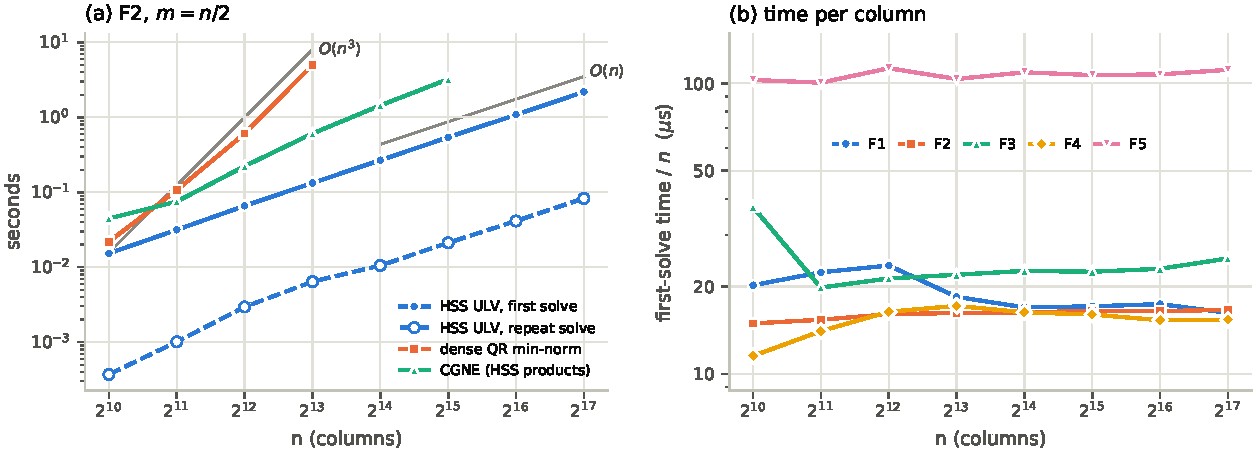
\includegraphics[width=\textwidth]{figures/m1_complexity.pdf}
\caption{Measured cost. (a) F2, $m=n/2$, rank 10: first solve (factorization and solve), repeat solve
with the stored factors, dense QR minimum-norm solve and CGNE (conjugate gradients on $HH^*$ with HSS
products, to relative residual $10^{-12}$); grey lines $O(n)$ and $O(n^3)$. (b) Time of the first solve
divided by $n$, for F1--F5: a flat line is linear cost (the first F3 point is a single dense block).
Times from \TimingPlatform; HSS solves are the median of three runs after a warm-up, each first solve
starting without stored factors; dense QR and CGNE are single runs.}
\label{fig:complexity}
\end{figure}


% ======================================================================
\section{Algorithm Summary}\label{sec:summary}
\begin{algorithm}[h]
\caption{Recursive Complete Minimum-Norm HSS Solve, $\mathcal M(H,b)$}
\label{alg:minnorm}
\begin{algorithmic}[1]
\Require HSS matrix $H\in\mathbb{C}^{m\times n}$, $m\le n$, full row rank, proper representation; $b\in\mathbb{C}^m$
\If{$H$ is a single dense block $D$}
  \State \Return $D^+b$ \Comment{from an SVD of $D$; $D^{-1}b$ if square}
\EndIf
\ForAll{leaves $\tau$}
  \State \textbf{if} $\ell_\tau+n_\tau<p_\tau$: $[V_\tau^*;D_\tau]\,\Omega_\tau=[\tilde V_\tau^*,0;\tilde D_\tau,0]$; \textbf{else} $\Omega_\tau=I$ \Comment{size reduction}
  \State $P_\tau^*U_\tau=[0;\hat U_\tau]$; \ $\tilde D_\tau\gets P_\tau^*\tilde D_\tau$; \ $\hat b_\tau=P_\tau^*b_\tau$ \Comment{row compression}
  \State $\tilde D_\tau(1{:}t_\tau,:)\,Q_\tau=[L_\tau,0]$; \ $\hat D_\tau=\tilde D_\tau Q_\tau$; \ $\hat V_\tau^*=\tilde V_\tau^*Q_\tau$ \Comment{column decoupling}
  \State $X^{(1)}_\tau=L_\tau^{-1}\hat b_\tau(1{:}t_\tau)$ \Comment{forced solve}
\EndFor
\State $\bar b\gets\big(\hat b-\hat H[X^{(1)};0]\big)(\mathcal R_2)$ \Comment{one HSS product, \eqref{eq:bbar}}
\State $\bar H\gets$ discard decoupled rows and forced columns, merge sibling leaves \eqref{eq:merge}
\State $\bar x\gets\mathcal M(\bar H,\bar b)$ \Comment{one level fewer}
\State \Return $x_\tau=\Omega_\tau\big[Q_\tau[X^{(1)}_\tau;\bar x_\tau];\,0\big]$ for every leaf
\end{algorithmic}
\end{algorithm}

% ======================================================================
\section{Numerical Experiments}\label{sec:numerics}

\subsection{Setup}\label{subsec:protocol}
Each subsection names the MATLAB test file that produces its results. The accuracy tests at moderate size
use leaves of 16--64 rows, so that every tree has 3--7 levels; the timing and large-$n$ runs use leaves of
200--400 rows. \PlatformSentence

With $x$ the computed solution, we report:
\begin{itemize}[leftmargin=1.5em,itemsep=1pt]
\item the residual $\|Hx-b\|/\|b\|$;
\item the \emph{solver error} $\|x-x_{\rm ref}\|/\|x_{\rm ref}\|$, where $x_{\rm ref}$ is the dense minimum-norm
solution of the HSS matrix itself, computed from a QR factorization $H^*=QR$ as $x_{\rm ref}=Q(R^{-*}b)$. This
measures the solver alone, without the compression error;
\item the error against the minimum-norm solution of the original matrix $A$, which adds the compression
error;
\item the null-space fraction $\|P_{\mathcal N(H)}x\|/\|x\|$, which is $0$ for an exact minimum-norm solution;
\item for large $n$, where no dense matrix can be formed, the error against a \emph{manufactured}
solution: draw $z$, set $x_\star=H^*z$ and $b=Hx_\star$. Since $x_\star\in\operatorname{Range}(H^*)$ and
$Hx_\star=b$, $x_\star$ \emph{is} $H^+b$, and $\|x-x_\star\|/\|x_\star\|$ needs only HSS products.
\end{itemize}

\subsection{Test matrices}\label{subsec:testmatrices}
Table~\ref{tab:families} defines the families. F1 and F2 are given directly by their generators, so they
are exactly HSS; F3--F6 are compressed from their entries with nested interpolative decompositions.
Large-$n$ cases never form a dense matrix.

\begin{table}[!htb]
\centering\footnotesize
\setlength{\tabcolsep}{4pt}
\begin{tabular}{@{}l>{\raggedright\arraybackslash}p{8.4cm}>{\raggedright\arraybackslash}p{3.3cm}>{\raggedright\arraybackslash}p{1.9cm}@{}}
\toprule
& definition & HSS form & $\kappa$\\
\midrule
F1 & $A=XY+\operatorname{blkdiag}(E_\tau)$, $X\in\mathbb{R}^{m\times k}$, $Y\in\mathbb{R}^{k\times n}$, $E_\tau\in\mathbb{R}^{n_\tau\times p_\tau}$ (one block per leaf), entries iid $U[0,1]$ & exact, rank $k$ ($U_\tau=X(I_\tau,:)$, $V_\tau=Y(:,J_\tau)^T$, $R=W=[I;I]$, $B=I$) & \KFone, grows $\propto n$\\
F2 & random HSS: $D_\tau$ iid $N(0,1)/\sqrt{p_\tau}$; $U,V,R,W$ with orthonormal columns (QR of Gaussian matrices); $B$ iid $N(0,1)/\sqrt k$; real or complex & exact, rank $k$ & \KFtwo\\
F2$_\alpha$ & F2 with graded columns: $H\operatorname{diag}(10^{-\alpha u_j})$, $u_j$ iid $U[0,1]$, $\alpha\ge0$ & exact, same ranks as F2 & \KFtwoG\\
F3 & $A_{ij}=1/(x_i-y_j)$, $x_i=i$ ($i\le M$), three points $y=x_i+q/4$ ($q=1,2,3$) in each gap; $n=3(M-1)$ & tolerance $10^{-10}$ & \KFthree\\
F4 & $y_i=\sum_jg(si+w-j)\,x_j$: Gaussian (width $\sigma$) or Ricker wavelet $g$, truncated at $|d|\le w=\lceil4\sigma\rceil$; stride $s$; ``valid'' outputs only & exact (banded) & \KFfour, grows with $\sigma$\\
F5 & $C=AF^*$ with $A_{jk}=e^{2\pi ikx_j}$, $k=-N/2,\dots,N/2-1$, jittered $x_j$, $F$ the unitary DFT: $C_{jl}=D_N(x_j-l/N)/\sqrt N$, $D_N$ the Dirichlet kernel; complex & tolerance $10^{-12}$ & \KFfive\\
F6 & $C=F_mTD^*F_n^*$ with $T\in\mathbb{R}^{m\times 2m}$ random Toeplitz, $F_m,F_n$ unitary DFTs, $D$ a unit-modulus diagonal & tolerance $10^{-12}$ & \KFsix\\
\bottomrule
\end{tabular}
\caption{Test families. All are wide ($m<n$) and of full row rank. $\kappa$ at the sizes of Table~\ref{tab:e1}
(F2$_\alpha$ and F4: over the sweeps of Section~\ref{subsec:stab}).}
\label{tab:families}
\end{table}

\paragraph{Notes on the families.}
F1 has a rank-$k$ part with all-positive entries. Its largest singular value is therefore about
$\tfrac k4\sqrt{mn}$, far above the rest of the spectrum, so $\kappa(\mathrm{F1})$ grows linearly with $n$,
and so does the error at large $n$ (Section~\ref{subsec:large}). F2 is the generic case: fixed rank and
a small condition number. Scaling its columns (F2$_\alpha$) keeps it exactly HSS with the same ranks and raises
$\kappa$ steadily with $\alpha$ (roughly like $10^{\alpha/2}$), which makes $\kappa$ a parameter. F3 is a smooth kernel matrix;
interlacing the two point sets keeps $\kappa\approx2$ at every size. F4 is a decimated convolution, as in
deconvolution with a ``valid'' boundary or a stride: it is banded and therefore exactly HSS, and its
condition number is set by the blur width $\sigma$. We use it to compare the direct solver with
iterative methods as $\kappa$ grows (Section~\ref{subsec:stab}). F5 and F6 come from matrices that are not
HSS themselves: a nonuniform Fourier matrix, as in interpolating a band-limited signal from irregular
samples, and a random Toeplitz matrix, whose off-diagonal blocks have full rank. Unitary DFTs turn both
into Cauchy-like matrices, which are HSS~\cite{gko}. By Lemma~\ref{lem:twosided}, a unitary change of
variables maps minimum-norm solutions to minimum-norm solutions, so the solver applies to the transformed
system unchanged.

\subsection{Correctness at moderate size}\label{subsec:correct}
Table~\ref{tab:e1} runs every family at a size where the dense references are affordable
(\texttt{mp\_exp\_correctness.m}). In every case the residual is at most $\EoneMaxRes$ and the solver error is at most
$\EoneMaxErrOverKappaU\,\kappa(H)u$\EoneSmallKappaClause. The null-space fraction, the part of $x$ that a minimum-norm solution
must not have, is of the same size as the solver error; a method that solved $Hx=b$ but drifted from the
minimum-norm solution would show a null-space fraction far above the residual. The error against the
original matrix adds the compression error: for F3, F5 and F6 it is $\EoneCompMin$--$\EoneCompMax$, of
the size of the compression tolerance ($10^{-10}$ for F3, $10^{-12}$ for F5 and F6), as the
$2\kappa\varepsilon$ bound of Section~\ref{sec:proof} predicts; for F1, F2 and F4, which are exactly HSS, it
agrees with the solver error.
The cases \EoneNoSlack{} violate the slack condition of Assumption~\ref{as:slack} and are as accurate as
the others.

\begin{table}[!htb]
\centering\scriptsize
\setlength{\tabcolsep}{3pt}
\begin{tabular}{@{}lrrrrrcccccc@{}}
\toprule
case & $m$ & $n$ & $L$ & rank & $\kappa(H)$ & As.~\ref{as:slack} & residual & solver error & null frac. & vs.\ $A$\\
\midrule
F1 & 320 & 480 & 4 & 3 & $1.3{\times}10^{3}$ & yes & $5.9{\times}10^{-15}$ & $2.3{\times}10^{-14}$ & $1.6{\times}10^{-14}$ & $2.3{\times}10^{-14}$\\
F1 & 2048 & 4096 & 7 & 3 & $7.4{\times}10^{3}$ & yes & $2.8{\times}10^{-14}$ & $1.9{\times}10^{-13}$ & $1.7{\times}10^{-13}$ & $1.9{\times}10^{-13}$\\
F2 & 1024 & 2048 & 5 & 10 & 14 & yes & $1.4{\times}10^{-15}$ & $3.6{\times}10^{-15}$ & $3.2{\times}10^{-15}$ & $3.6{\times}10^{-15}$\\
F2 complex & 1024 & 2048 & 5 & 10 & 13 & yes & $1.5{\times}10^{-15}$ & $5.2{\times}10^{-15}$ & $4.6{\times}10^{-15}$ & $5.2{\times}10^{-15}$\\
F2 $m/n=0.9$ & 1800 & 2000 & 5 & 8 & 79 & no & $2.5{\times}10^{-15}$ & $1.4{\times}10^{-14}$ & $1.2{\times}10^{-14}$ & $1.4{\times}10^{-14}$\\
F3 & 1024 & 3069 & 5 & 32 & 1.9 & yes & $1.1{\times}10^{-15}$ & $2.2{\times}10^{-15}$ & $2.2{\times}10^{-15}$ & $6.7{\times}10^{-11}$\\
F4 Gaussian, $\sigma=2$, $s=2$ & 2040 & 4096 & 5 & 10 & 98 & yes & $6.6{\times}10^{-15}$ & $1.0{\times}10^{-14}$ & $8.7{\times}10^{-15}$ & $1.0{\times}10^{-14}$\\
F4 Ricker, $\sigma=3$, $s=2$ & 2036 & 4096 & 5 & 15 & $2.2{\times}10^{3}$ & yes & $7.7{\times}10^{-14}$ & $1.9{\times}10^{-13}$ & $1.9{\times}10^{-13}$ & $2.0{\times}10^{-13}$\\
F4 Gaussian, $\sigma=3$, $s=3$ & 1358 & 4096 & 5 & 10 & 98 & yes & $5.1{\times}10^{-15}$ & $1.0{\times}10^{-14}$ & $9.3{\times}10^{-15}$ & $1.0{\times}10^{-14}$\\
F5 & 1536 & 2048 & 5 & 36 & 2.0 & no & $1.2{\times}10^{-15}$ & $3.1{\times}10^{-15}$ & $3.1{\times}10^{-15}$ & $1.0{\times}10^{-12}$\\
F6 & 1024 & 2048 & 5 & 62 & 7.4 & no & $2.1{\times}10^{-15}$ & $4.2{\times}10^{-15}$ & $3.7{\times}10^{-15}$ & $1.4{\times}10^{-12}$\\
\bottomrule
\end{tabular}

\caption{Accuracy at moderate size. ``rank'': largest generator rank; $L$: depth; ``As.~\ref{as:slack}'':
whether every leaf satisfies the slack condition. ``vs.\ $A$'': error against the minimum-norm solution
of the original matrix (for F6, in the Toeplitz variables, $x=D^*F_n^*y$).}
\label{tab:e1}
\end{table}

\subsection{Accuracy as the condition number grows}\label{subsec:stab}
Figure~\ref{fig:stab} sweeps $\kappa(H)$ in the two families where it is a parameter, F2$_\alpha$ (depth 3)
and F4 with stride 1 and growing $\sigma$ (depth 4), and compares the ULV solve with the normal equations
(Cholesky factorization of $HH^*$) and with CGNE (conjugate gradients on $HH^*$ with HSS products,
relative-residual tolerance $10^{-14}$, at most 2000 iterations). All are measured against the dense QR
solution (\texttt{mp\_exp\_conditioning.m}). For an ill-conditioned problem that reference is itself
accurate only to about $\kappa u$ ($u\approx1.1\times10^{-16}$), so differences below $\kappa u$ cannot be
resolved: a curve at or below the $\kappa u$ line means the method is as accurate as dense QR.

The ULV solution stays within $\EtwoUlvOverKappaU\,\kappa u$ of the dense QR solution over the whole range,
up to $\kappa\approx\EtwoMaxKappaGraded$ for F2$_\alpha$ and $\EtwoMaxKappaBlur$ for F4: it is as accurate as
dense QR. The normal equations follow $\kappa^2u$, as squaring the condition number predicts, and their
Cholesky factorization fails from $\kappa\approx\EtwoCholFailGraded$ (F2$_\alpha$) and $\EtwoCholFailBlur$ (F4) on.
CGNE needs $\EtwoCgItsMinGraded$ iterations already at $\kappa\approx10$; from $\kappa\approx\EtwoCgFailGraded$
(F2$_\alpha$) and $\EtwoCgFailBlur$ (F4) on it does not converge within 2000 iterations and its error exceeds
$10^{-6}$. This is the regime that needs a direct solver. The backward error
$\|b-Hx\|/(\|H\|\|x\|+\|b\|)$, which needs no reference, is the smallest relative perturbation of $H$ and
$b$ for which $x$ solves the system exactly; it stays below $\EtwoUlvBwdMax$ for the ULV solution throughout
(dense QR: $\EtwoQrBwdMax$) and grows to $\EtwoNeBwdMax$ for the normal equations.

\begin{figure}[!htb]
\centering
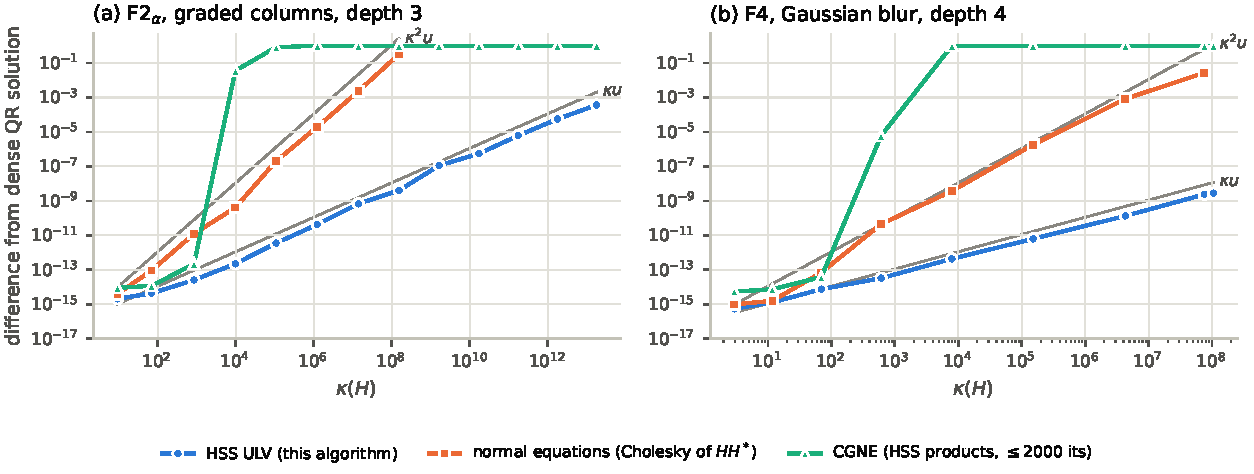
\includegraphics[width=\textwidth]{figures/m1_stability.pdf}
\caption{Relative difference from the dense QR minimum-norm solution as $\kappa(H)$ grows. (a) F2$_\alpha$,
$128\times256$, depth 3; (b) F4, Gaussian blur, stride 1, $\approx290\times300$, depth 4. Grey lines:
$\kappa u$ and $\kappa^2u$. Missing normal-equation points: the Cholesky factorization of $HH^*$ failed.
CGNE values of 1: no iterate had a smaller residual than the starting guess $0$, which is returned.}
\label{fig:stab}
\end{figure}

\subsection{Accuracy at large $n$}\label{subsec:large}
With manufactured solutions the solver can be checked at sizes where no dense matrix fits
(Figure~\ref{fig:largescale}, \texttt{mp\_exp\_scaling.m}, the same run as Figure~\ref{fig:complexity}).
For F2--F5 the error stays between $\EthreeErrMin$ and $\EthreeErrMax$ for every $n$ up to $\EfourMaxN$.
For F1 it grows from $\EthreeFoneFirst$ to $\EthreeFoneLast$, in step with $\kappa(\mathrm{F1})\propto n$
(Section~\ref{subsec:testmatrices}): this is the conditioning of the test matrix, not error growth in the
solver. Residuals are at most $\EthreeMaxRes$.

\begin{figure}[!htb]
\centering
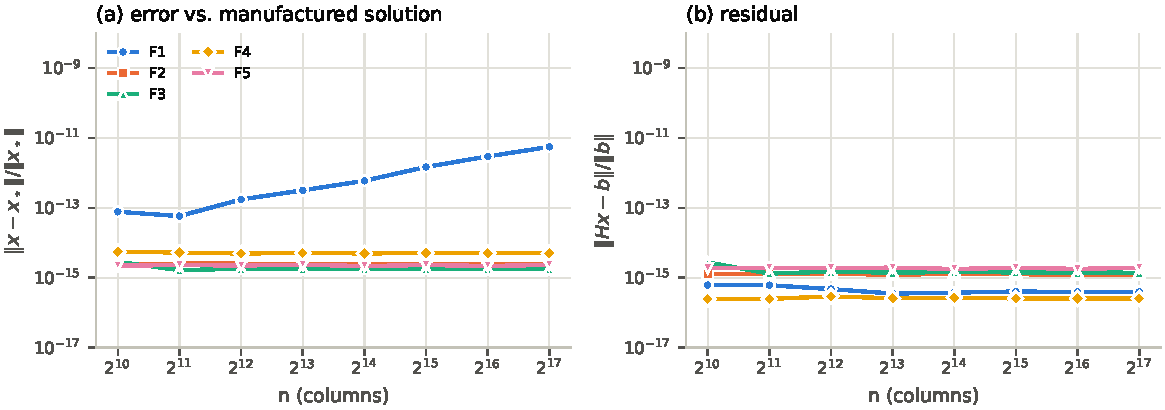
\includegraphics[width=0.92\textwidth]{figures/m1_largescale_accuracy.pdf}
\caption{Error against the manufactured minimum-norm solution as $n$ grows. No dense matrix is formed.}
\label{fig:largescale}
\end{figure}


% ======================================================================
\section{Open Problems}\label{sec:open}
\begin{enumerate}[leftmargin=1.5em,itemsep=2pt]
\item \textbf{Floating-point analysis.} The experiments are consistent with backward stability, but there
is no proof. A natural route is the backward-error analysis of ULV for square HSS matrices, extended by the
size reduction.
\item \textbf{Leaf size.} The cost model of Section~\ref{sec:complexity} is smallest for leaves of about $r$
rows; choosing the leaf size from the ranks, instead of fixing it, should lower the constant.
\item \textbf{Rank-deficient $H$.} The reduction is exact only for full row rank. Extending it to the
minimum-norm least-squares solution would cover inconsistent and rank-deficient systems.
\item \textbf{Higher dimensions.} For 2-D and 3-D problems the HSS ranks grow with the size of the
interfaces between clusters; formats with strong admissibility ($\mathcal H^2$, recursive
skeletonization) are needed, and the reduction of Section~\ref{sec:algorithm} should carry over block by
block.
\end{enumerate}

\begin{thebibliography}{9}\small
\bibitem{cgp} S.~Chandrasekaran, M.~Gu, T.~Pals, A fast ULV decomposition solver for hierarchically
semiseparable representations, \emph{SIAM J. Matrix Anal. Appl.} 28 (2006).
\bibitem{dh} J.~Demmel, N.~J.~Higham, Improved error bounds for underdetermined system solvers,
\emph{SIAM J. Matrix Anal. Appl.} 14 (1993).
\bibitem{gko} I.~Gohberg, T.~Kailath, V.~Olshevsky, Fast Gaussian elimination with partial pivoting
for matrices with displacement structure, \emph{Math. Comp.} 64 (1995).
\bibitem{higham} N.~J.~Higham, \emph{Accuracy and Stability of Numerical Algorithms}, 2nd ed., SIAM,
2002.
\end{thebibliography}
\end{document}
